I% Chapter Template

\chapter{Vector Structure} % Main chapter title

\label{VectorStructure} % Change X to a consecutive number; for referencing this chapter elsewhere, use \ref{ChapterX}

\lhead{Vector Structure. \emph{Vector Structure}} % Change X to a consecutive number; this is for the header on each page - perhaps a shortened title

%----------------------------------------------------------------------------------------
%	SECTION - Radix Balanced Vectors
%----------------------------------------------------------------------------------------

\section{Radix Balanced Vectors}

%-----------------------------------
%	SUBSECTION - Tree structure
%-----------------------------------

\subsection{Tree structure}
% describe tree: balancing, filling, block sizes
% why structure helps with operations implementation 
% hint why radix?  


\begin{figure}[h!]
  \centering
  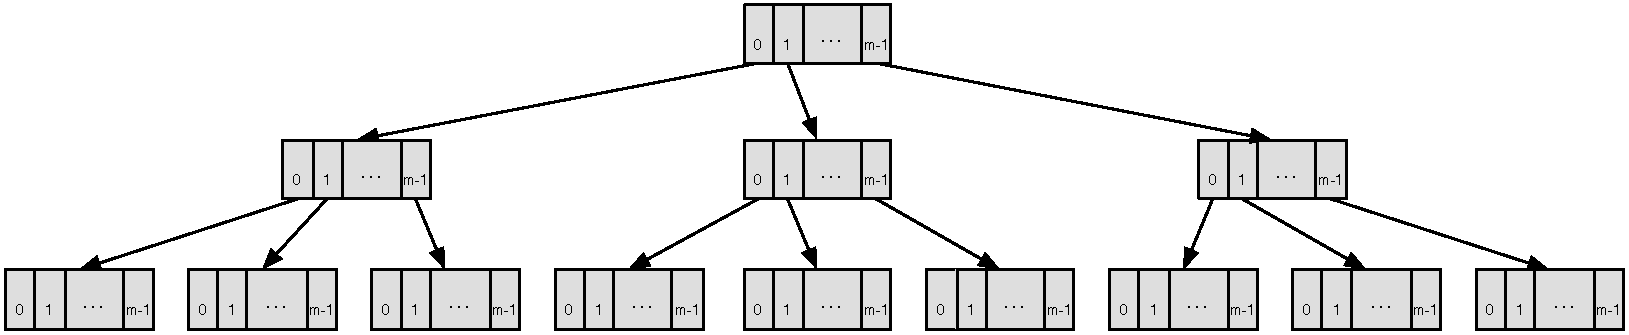
\includegraphics[width=\textwidth]{Figures/Radix_Balanced}
  \label{badix_balanced}
  \caption{Radix Balanced Tree Structure}
\end{figure}



%-----------------------------------
%	SUBSECTION - Operations
%-----------------------------------
\subsection{Operations}
% List core operations
% Hint of displays and transient states


%-----------------------------------
%	SUBSUBSECTION - Apply
%-----------------------------------

\subsubsection{Apply}
% used in head and last
% performance log_32(n), hint of displays

%-----------------------------------
%	SUBSUBSECTION - Updated
%-----------------------------------

\subsubsection{Updated}
% base implementation needs to update the whole branch

% with transient states, local updates can be amortised

%-----------------------------------
%	SUBSUBSECTION - Additions
%-----------------------------------

\subsubsection{Additions}

\paragraph{Append}
% base implementation needs to update the whole branch
% performance log_32(n), hint of transient to amortise consecutive appends are amortised

\paragraph{Prepend}
% base implementation needs to update the whole branch
% shift top and start index
% performance log_32(n), hint of transient to amortise consecutive appends are amortised

\paragraph{Concatenation and Insert}
% describe high level implementation in vector
%% describe branch rebalancing 
% performance O(n)


%-----------------------------------
%	SUBSUBSECTION - Splits
%-----------------------------------

\subsubsection{Splits}
% used in tail, init, take, takeRight, drop, dropRight
% describe implementation in vector
% performance log_32(n) 


%----------------------------------------------------------------------------------------
%	SECTION - Parallel Vectors
%----------------------------------------------------------------------------------------

\section{Parallel Vectors}



%-----------------------------------
%	SUBSUBSECTION - Splitter
%-----------------------------------

\subsection{Splitter Iterator}



%-----------------------------------
%	SUBSUBSECTION - Combiner
%-----------------------------------

\subsection{Combiner Builder}



%----------------------------------------------------------------------------------------
%	SECTION - Relaxed Radix Balanced Vectors
%----------------------------------------------------------------------------------------

\section{Relaxed Radix Balanced Vectors}

%-----------------------------------
%	SUBSECTION - Tree structure
%-----------------------------------

\subsection{Relaxed Tree structure}
% describe tree: balancing, filling, block sizes
% describe sizes array and where it is kept (change from left to right for indexing simplification)
% mention size of nodes and null sizes
% unbalanced trees can only be generated by concatenation, and splits

\begin{figure}[h!]
  \centering
  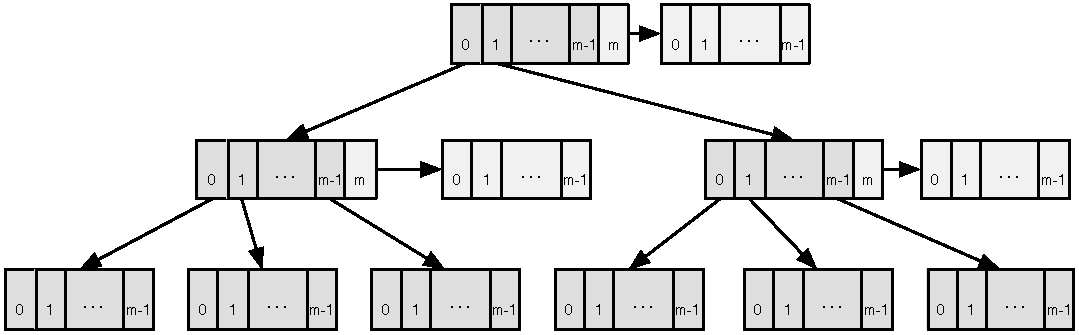
\includegraphics[width=\textwidth]{Figures/Relaxed_Radix_balanced}
  \label{Relaxed_Radix_balanced}
  \caption{Radix Balanced Tree}
\end{figure}

\begin{figure}[h!]
  \centering
  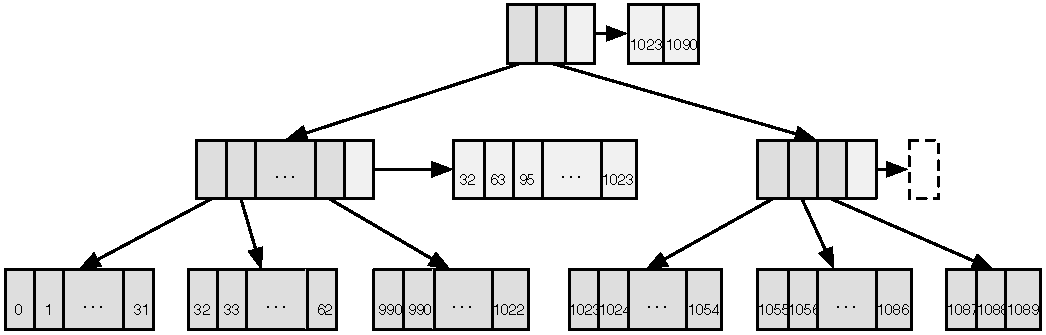
\includegraphics[width=\textwidth]{Figures/Relaxed_radix_example}
  \label{Relaxed_radix_example}
  \caption{Relaxed radix example}
\end{figure}

%-----------------------------------
%	SUBSECTION - Operations
%-----------------------------------
\subsection{Relaxed Operations}
% describe how the implementation uses relaxed radix when necessary and uses radix based operation when possible

%-----------------------------------
%	SUBSUBSECTION - Apply
%-----------------------------------

\subsubsection{Apply (get element at index)}
% describe the way to get the node indices in an unbalanced node


%-----------------------------------
%	SUBSUBSECTION - Updated
%-----------------------------------

\subsubsection{Updated}
% doesn't change much, the sizes do not need to be updated, they jus need to be copied. Going to the correct position still may needs to access the sizes.

%-----------------------------------
%	SUBSUBSECTION - Additions
%-----------------------------------

\subsubsection{Additions}

%-----------------------------------
\paragraph{Append}
% difference is that the the sizes may need to be updated
% performance log_32(n), remind hint of transient to amortise consecutive appends are amortised

\paragraph{Prepend}
% describe different implementation
% hint the 


%-----------------------------------
\paragraph{Concatenation}
% describe high level implementation in rrbvector
%% describe branch rebalancing 
% performance log_32(n)

\begin{figure}[h!]
  \centering
  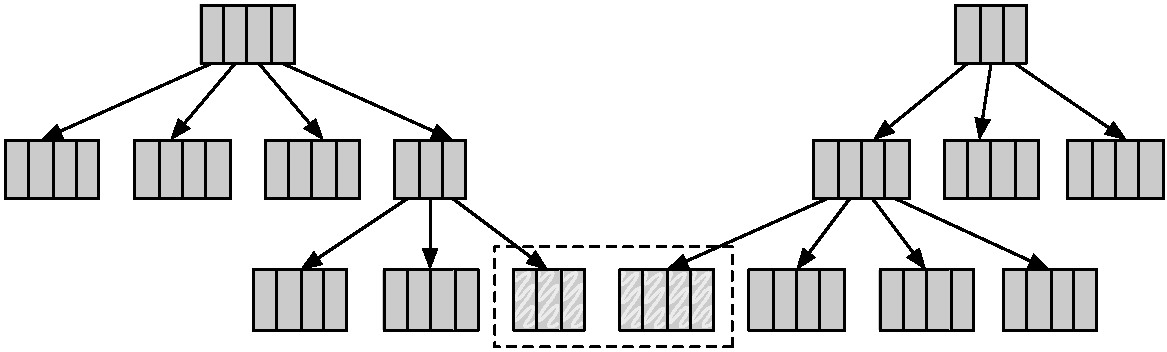
\includegraphics[width=\textwidth]{Figures/Concat0.pdf}
  \label{Concat0Benchmarks}
  \caption{Concatenation example with blocks of size 4: Rebalancing level 0}
\end{figure}

\begin{figure}[h!]
  \centering
  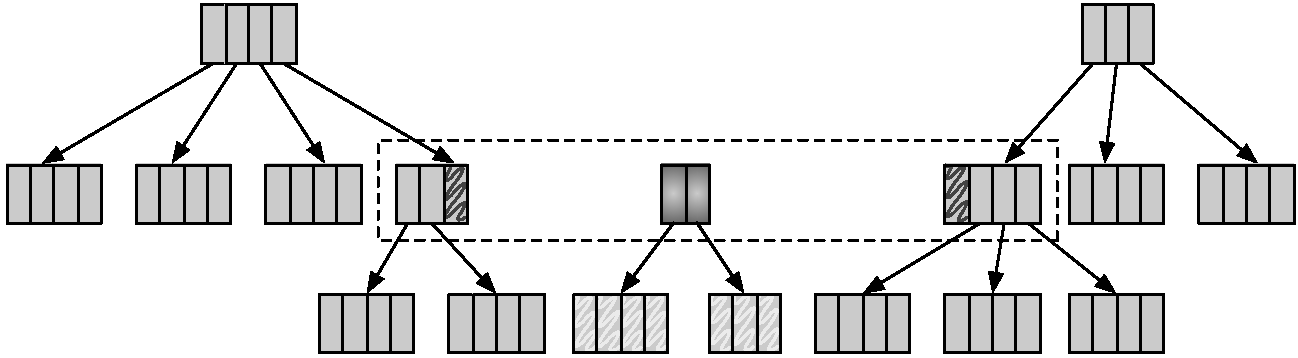
\includegraphics[width=\textwidth]{Figures/Concat1.pdf}
  \label{Concat1Benchmarks}
  \caption{Concatenation example with blocks of size 4: Rebalancing level 1}
\end{figure}

\begin{figure}[h!]
  \centering
  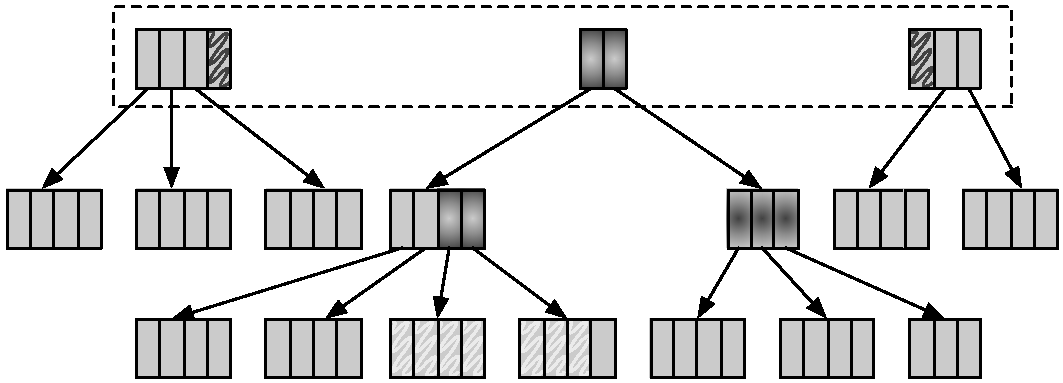
\includegraphics[width=\textwidth]{Figures/Concat2.pdf}
  \label{Concat2Benchmarks}
  \caption{Concatenation example with blocks of size 4: Rebalancing level 2}
\end{figure}

\begin{figure}[h!]
  \centering
  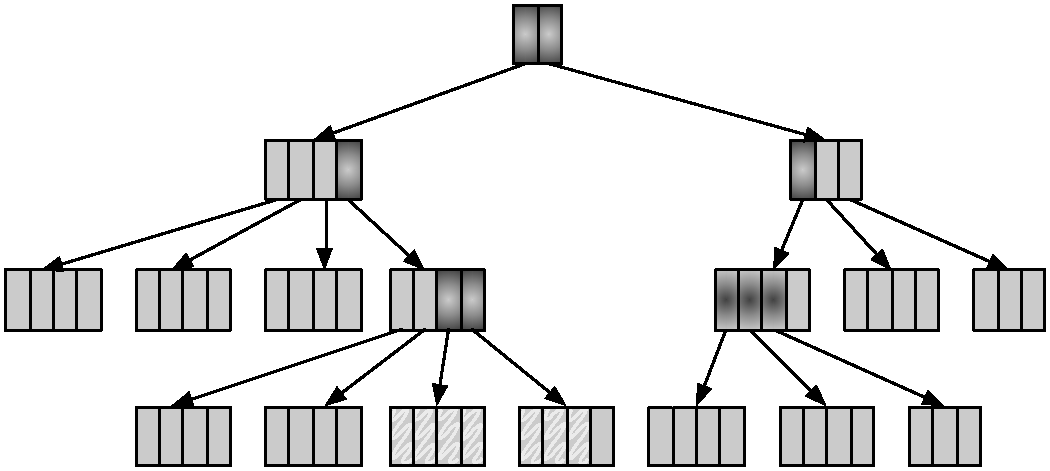
\includegraphics[width=\textwidth]{Figures/Concat3.pdf}
  \label{Concat3Benchmarks}
  \caption{Concatenation example with blocks of size 4: Rebalancing level 3}
\end{figure}


%-----------------------------------
\paragraph{Insert}
% new operation
% describe simple implementation using split and concat 
% performance log_32 (from split + concat)
% hint at possible optimization by inserting directly and using transient states (take advantage of locality)



%-----------------------------------
%	SUBSUBSECTION - Splits
%-----------------------------------

\subsubsection{Splits}
% used in tail, init, take, takeRight, drop, dropRight
% describe difference between the implementation (null and shift vs. cut and update size)


